\enteteExam{NFP 107 -- Systèmes de gestion de bases de données - Durée 2h30}%
{Première session --  26 janvier 2022}%
{Effectué à distance}%

\vspace{1ex}

Le schéma de base de données suivant sera utilisé pour l'ensemble du
sujet. Il permet de gérer les souscriptions pour un ensemble 
d'opérateurs de téléphonie mobile. Ce schéma sera nommé \textbf{schéma final} 
par la suite.

\begin{itemize}
 \item Opérateur (\textbf{id}, nom)
 \item Forfait (\textbf{id}, nom, idOpérateur, prix)
 \item Client(\textbf{id}, nom, prénom, ville)
 \item Souscription(\textbf{idClient, idForfait}, durée, numéro)
% \item Résiliation (id, dateResiliation, portabilité, idNouvelleSouscription)
\end{itemize}

L'attribut \texttt{durée} est un entier positif exprimant le nombre de mois d'engagement.
les clés étrangères ne sont pas indiquées.

\section{Conception (8 points}

La figure~\ref{forfait_telephone} montre une modélisation initiale de la 
base par un schéma entité association.


\begin{center}
  \begin{figure}[htb]  
   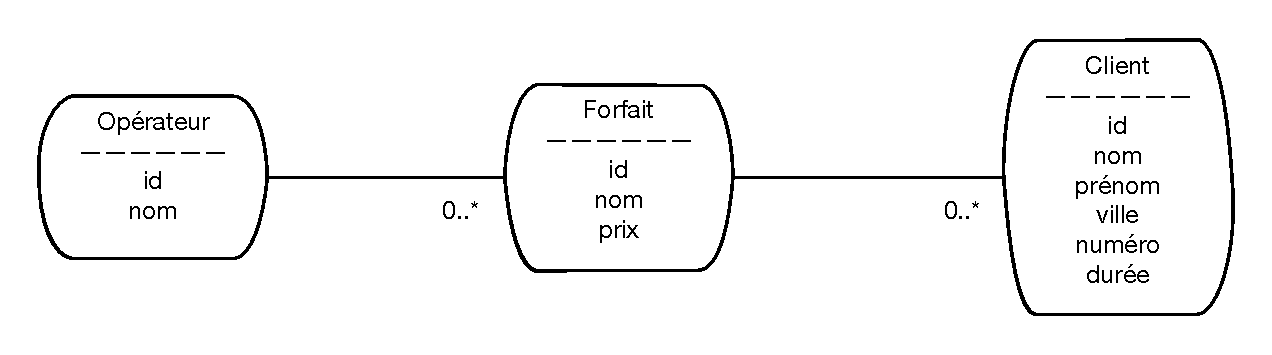
\includegraphics[scale=0.6]{../figures/forfait_telephone}
    \caption{Modélisation initiale de la base}  
    \label{forfait_telephone}  
  \end{figure}  
\end{center}

\begin{enumerate}
 \item Donnez la liste des dépendances fonctionnelles définies par ce schéma initial (1 pt)
  \item Donnez le schéma relationnel correspondant à la figure~\ref{forfait_telephone}, 
  sous forme simplifiée (Nom de table, 
  liste des attributs en encadrant les clés primaires et en soulignant les clés étrangères) (1 pt)
  \item Quelles sont les différences entre le schéma initial et le schéma final\,? À quelle(s)
       évolution(s) des choix de modélisation ce changement correspond-t-il (2 pts)\,? 
  \item Dessinez le schéma final sous forme entité-association. Quelles dépendances fonctionnelles ont changé
     par rapport au schéma initial\,? (1 pt)
  \item Dans le schéma final, une réification serait-elle possible\,? Quels changements impliquerait-elle\, (1 pt)?
  \item Donnez les commandes \texttt{create table} pour le schéma final (2 pts)
\end{enumerate}

\begin{solution}
  

\begin{center}
  \begin{figure}[htb]  
   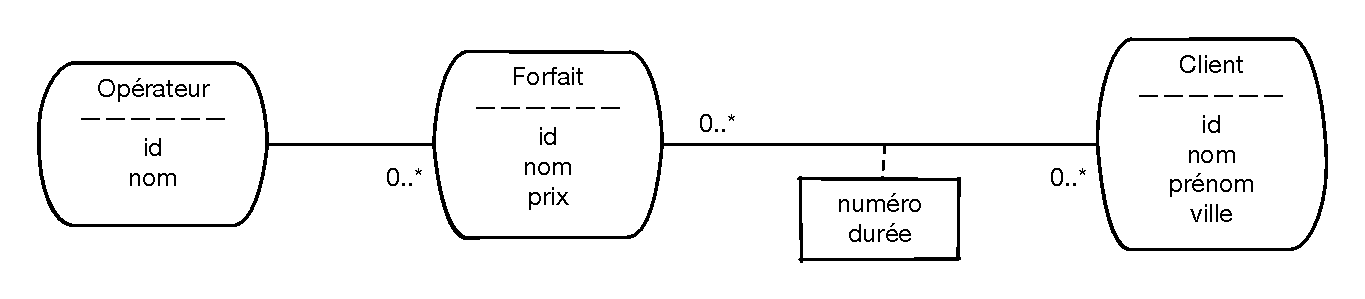
\includegraphics[scale=0.6]{../figures/forfait_telephone_final}
    \caption{Modélisation finale de la base}  
    \label{forfait_telephone_initial}  
  \end{figure}  
\end{center}


\begin{enumerate}
 \item \texttt{idOpérateur $\to$ nom} ; \texttt{idForfait $\to$ nom, prix, idOpérateur} ; \texttt{idClient $\to$ 
     nom, prénom, ville, numéro, durée}
 \item 
 
 
\begin{itemize}
 \item Opérateur (\textbf{id}, nom)
 \item Forfait (\textbf{id}, nom, \textit{idOpérateur}, prix)
 \item Client(\textbf{id}, nom, prénom, ville, durée, numéro, \textit{idForfait})
 \end{itemize}

  \item Dans le schéma initial, un client peut prendre un seul forfait, d'où
  la DF \texttt{idClient $\to$ idForfait}. Dans le schéma final un client peut prendre
     plusieurs forfaits (mais pas plusieurs fois le même), avec donc plusieurs numéros.
     
  \item Voir figure~\ref{forfait_telephone_initial}. Une nouvelle  clé est définie par 
  l'association plusieurs-plusieurs, avec la DF \texttt{idClient, idForfait $\to$ durée, numéro}
  \item En réifiant l'association  plusieurs-plusieurs, on attribuerait un identifiant propre
     à la souscription, et un même client pourrait prendre plusieurs fois le même forfait,
        ce qui n'est pas possible dans le schéma final. Dans une ``vraie'' base, ce seerait sans 
        doute souhaitable.
        
  \item Classique. La table \texttt{Souscription} est typique d'une association plusieurs-plusieurs.
  
\begin{minted}{sql} 
create table Souscription
   (idClient integer not null,
    idForfait varchar not null,
    durée integer not null,
    numéro integer not null,
     primary key(idClient, idForfait),
     foreign key (idClient) references Client (id),
     foreign key (idForfait) references Forfait (id));
\end{minted}
\end{enumerate}
  
\end{solution}



\section{SQL (7 points)}

Exprimez en SQL les requêtes suivantes \textbf{sur le schéma final, donné dans l'énoncé de l'examen.}

\begin{enumerate}

\item Nom et prénom des clients qui ont souscrit un forfait avec engagement de plus de 24 mois.

\begin{solution}
	\begin{minted}{sql}
	select c.nom, c.prenom
	from Client as c, Souscription as s
	where s.idClient = c.id and s.duree > 24;
	\end{minted}
\end{solution}

\item Existe-t-il deux clients qui auraient le même numéro de téléphone pour le même forfait\,? 
Donnez leurs noms et prénoms (des .clients)

\begin{solution}
	\begin{minted}{sql}
	select nom, c.prenom
	from Client as c1, Souscription as s1,
	      Client as c2, Souscription as s2
	where c1.id = s1.idClient,
	and c2.id = s2.idClient 
	and s1.idForfait = s2.idForfait
	and c1.numéro = c2.numéro
	\end{minted}
\end{solution}


\item Noms des clients qui ont un forfait nommé \emph{Audace} et un autre nommé   \emph{Privilège}
     \emph{Libre} 
 
 
\begin{solution}
	\begin{minted}{sql}
	select nom, c.prenom
	from Client as c, Souscription as s1, Souscription as s2,
	       Forfait as f1, Forfait as f2
	where c.id = s1.idClient,
	and c.id = s2.idClient 
	and s1.idForfait = f1.idForfait
	and s2.idForfait = f2.idForfait
	and f1.nom='Audace' and f2.nom='Privilège'
	\end{minted}
\end{solution}

 \item Quels clients n'ont pas souscrit de forfait\,?

\begin{solution}
	\begin{minted}{sql}
	select c.nom, c.prenom
	from Client as c 
	where not exists 
	    (select * from Souscription as s 
	         where c.id = s.idClient)
	\end{minted}
\end{solution}

\item Quels opérateurs n'ont pas de client à Lyon\,?


\begin{solution}
	\begin{minted}{sql}
	select o.nom
	from Opérateur as o
	where not exists 
	    (select * from Forfait as f, Souscription as s, Client as c
	         where o.id=f.idOpérateur
	         and   f.id=s.idForfait
	         and   s.idClient=c.id
	         and  c.ville='Lyon')
	\end{minted}
\end{solution}

\item Donnez le nombre de souscriptions pour chaque forfait de l'opérateur \emph{Violet}.

\begin{solution}
	\begin{minted}{sql}
	select f.nom, count(*) as nbSouscriptions
	from Opérateur as o, Forfait as f, Souscription as s
	where o.id=f.idOpérateur
	and   f.id=s.idForfait
	and   o.nom='Violet'
	group by f.id, f.nom
	\end{minted}
\end{solution}


\item Quels clients ont deux souscriptions  ou plus\,? Donnez le nombre de souscriptions.

\begin{solution}
	\begin{minted}{sql}
	select c.nom, c.prénom, count(*) as nbSouscriptions
	from Client as c, Souscription as s
	where c.id=s.idClient
	group by c.id, c.nom
	having count(*) > 1
	\end{minted}
\end{solution}
 
\end{enumerate}

\section{Algèbre relationnelle (3 pts)}

\begin{enumerate}
\item Expliquez ce que fait la requête algébrique suivante, et donnez une expression SQL équivalente
	$$\pi_{nom, prenom}(\sigma_{ville='Paris'}(Client) \underset{id=idClient}{\bowtie} (\sigma_{duree > 24}(Souscription) \underset{idForfait=id}{\bowtie} \sigma_{nom='\rm{Audace}'} (Forfait))$$


\item Même question pour l'expression suivante
	$$\pi_{c.id, c.nom, c.prenom} (Client) - \pi_{c.id, c.nom, c.prenom} (Client \underset{c.id=s.idClient}{\bowtie}\\ \sigma_{duree \geq 48} (Souscription))$$


\begin{solution}
Les clients qui n'ont pas de souscription supérieure à 48 mois.
\end{solution}
 
\item Voici une expression SQL ``algébrique''
\begin{minted}{sql}
select c.nom, c.prénom
from (Client as c join Souscription as s on c.id=s.idClient) 
        join (select * from Forfait as f where nom= 'Audace') 
                 on s.idForfait = f.id
\end{minted}

Donnez une expression SQL ``déclarative'' équivalente, et sans requête imbriquée.

\end{enumerate}

\section{Jointure externe (2 pts)}

Que renvoie la requête suivante\,? 
\begin{minted}{sql}
select c.nom, c.prénom, f.nom
from (Client as c outer join (Souscription as s join Forfait as f 
                                     on s.idForfait=f.id)
            on c.id = s.idClient
where ville= 'Nantes'
\end{minted}


\begin{solution}
On obtient tous les clients de Nantes, et leurs forfaits. Si un client n'a aucun forfait, une ligne
est produite quand même, avec le nom du forfait à \texttt{null}.
\end{solution}